\documentclass{beamer}

% Prepare for svenska tecken
\usepackage[T1]{fontenc}
\usepackage[utf8]{inputenc}
\usepackage[swedish]{babel}
%\usepackage[]{geometry}
\addto\captionsswedish{\renewcommand{\figurename}{Bild}}
\usepackage{amsmath}
\usepackage{fancyhdr}
\usepackage{wrapfig}
\usepackage{caption}
\usepackage{framed}
\usepackage[fulladjust]{marginnote}
\usepackage{color}
\newcommand{\hilight}[1]{\colorbox{yellow}{#1}}
\usepackage{hyperref}
\hypersetup{
    colorlinks,
    citecolor=black,
    filecolor=black,
    linkcolor=black,
    urlcolor=black
}
\usepackage{stmaryrd} % För symbolen \boxbox, kräver paketet texlive-math-extra

% % % % % % % % % % % 
% Detta är nya environments för review. De bör vara relativt självförklarande hur de används.
% I princip sätter man bara den del av texten som har en viss status mellan\begin{rev-granskat} och \end{rev-granskat} tex.
% Undvik att nästla dem för det är ingen idé det fungerar inte.
% De är testade med ett antal andra environemnt som tabular mm men kolla att det fungerar med de environments du använder.
% % % % % % % % % % % % % % % % % % % % % % % % % % % % % % % % % % % % % % % % % % % % % % % % % % % % % % % % % % % % % % % 
%\usepackage[svgnames,rgb]{xcolor}
%\usepackage{pdfcomment}
%\newenvironment{rev-ogranskat}{\begin{pdfsidelinecomment}[color=black,linewidth=3px,caption=inline]{Ogranskat}}{\end{pdfsidelinecomment}}
%\newenvironment{rev-omarbetas}{\begin{pdfsidelinecomment}[color=red,linewidth=3px,caption=inline]{Omarbetas}}{\end{pdfsidelinecomment}}
%\newenvironment{rev-raderas}{\begin{pdfsidelinecomment}[color=red,linewidth=3px,caption=inline]{Raderas}}{\end{pdfsidelinecomment}}
%\newenvironment{rev-redo}{\begin{pdfsidelinecomment}[color=yellow,linewidth=3px,caption=inline]{Redo att granska}}{\end{pdfsidelinecomment}}
%\newenvironment{rev-granskat}[1][]%
%{\begin{pdfsidelinecomment}[color=green,linewidth=3px,caption=inline]%
%{Granskat #1}}%
%{\end{pdfsidelinecomment}}
%\newenvironment{rev-nytt}[1][]%
%{\begin{pdfsidelinecomment}[color=brown,linewidth=3px,caption=inline]%
%{Nytt #1}}%
%{\end{pdfsidelinecomment}}
%\newenvironment{rev-releasat}{\begin{pdfsidelinecomment}[color=blue,linewidth=3px,caption=inline]{Klart}}{\end{pdfsidelinecomment}}

%\clubpenalty=9990
%\widowpenalty=9999
%\brokenpenalty=4999

\usepackage[europeanvoltages,europeancurrents,europeanresistors,cuteinductors,smartlabels]{circuitikz}
\usepackage[framemethod=TikZ]{mdframed}

\mdfdefinestyle{FactBox}{%
    linecolor=blue,
    outerlinewidth=2pt,
    roundcorner=20pt,
    innertopmargin=\baselineskip,
    innerbottommargin=\baselineskip,
    innerrightmargin=20pt,
    innerleftmargin=20pt,
    backgroundcolor=gray!50!white}
\newcommand{\infobox}[1]{
\begin{wrapfigure}{r}{0.5\textwidth}
  \begin{mdframed}[style=FactBox]
#1
  \end{mdframed}
\end{wrapfigure}
}

% Make some unicode characters usable
%\DeclareUnicodeCharacter{00B0}{\ensuremath{^\circ}} % unicode 00B0 ° degree sign
%\DeclareUnicodeCharacter{00B5}{\ensuremath{\mu}} % unicode 00B5 µ micro sign
%\DeclareUnicodeCharacter{03C0}{\ensuremath{\pi}} % unicode 3C0 π greek small letter pi
%\DeclareUnicodeCharacter{03A9}{\ensuremath{\Omega}} % unicode 3A9 Ω greek capital letter omega
%\DeclareUnicodeCharacter{2206}{\ensuremath{\Delta}} % unicode 2206 ∆ increment


% Prepare for tables
\usepackage{multirow}
\usepackage{xtab}

% Prepare for lists
%\usepackage{enumitem}

% Prepare for graphics
\usepackage{graphicx}

\raggedbottom


%% Frontpage bacground
\usepackage{eso-pic}
\newcommand\BackgroundPic{%
\put(0,0){%
\parbox[b][\paperheight]{\paperwidth}{%
\vfill
\centering
\includegraphics[width=\paperwidth,height=\paperheight,%
keepaspectratio]{images/koncept-front.jpg}%
\vfill
}}}


\newcommand\BackgroundPicLast{%
\put(0,0){%
\parbox[b][\paperheight]{\paperwidth}{%
\vfill
\centering
\includegraphics[width=\paperwidth,height=\paperheight,%
keepaspectratio]{images/koncept-back.pdf}%
\vfill
}}}

\usepackage[swedish]{babel}
\usepackage{lmodern}
\mode<presentation>
{
\usetheme{Madrid}
\usecolortheme{default}
\usefonttheme{serif}
\setbeamertemplate{navigation symbols}{}
\setbeamertemplate{caption}[numbered]
}
\usepackage{tikz}
\usepackage{amsmath,amsfonts,amssymb,bm,mathrsfs}
\usetikzlibrary{shapes,arrows}
\usepackage{siunitx}
\sisetup{
output-decimal-marker = {,},
per-mode=symbol,
range-units=single,
range-phrase={--}
}

\title[SM7NTJ]{Elektromagnetiska fält EMF}
\author{SSA utbildning}

\begin{document}

\begin{frame}
\titlepage
\includegraphics[height=0.3\textheight]{images/ssalogo}
\end{frame}

\begin{frame}{Innehåll}
\tableofcontents
\end{frame}

\section{Fält}

\begin{frame}{Elektriskt fält}

\begin{itemize}
	\item Mellan två ledare med elektrisk potentialskillnad	skapas ett
	elektriskt fält
	\item Elektrisk fältstyrka $E$ mäts i ''volt per meter'' [V/m] 
\end{itemize}
\end{frame}

\begin{frame}{Magnetiskt fält}

  \begin{itemize}
  	\item Runt en strömförande ledare skapas ett magnetiskt fält
  	\item Magnetisk fältstyrka $H$ mäts i ''ampere per meter'' [A/m]
  \end{itemize}
\end{frame}

\begin{frame}{Det elektromagnetiska fältet}
På ett visst avstånd från en antenn så sammanfaller det elektriska och det
magnetiska fälten till ett elektromagnetiskt fält.

\begin{itemize}
	\item Närfältet, är ett område nära antennen där fälten turas om att
	dominera. Lokala toppar kan uppstå och beräkning av fältstyrka är
	komplicerad
	\item Fjärrfältet, börjar normalt räknas på avståndet $\dfrac{\lambda}{6}$
	från antennen.
\end{itemize}
\end{frame}

\begin{frame}{Fjärrfältet}
Inom fjärrfältet
\begin{itemize}
	\item kan fältstyrkorna relativt enkelt beräknas
	\item avtar fältstyrkan linjärt med avståndet.\\
	(Detta gäller för både rundstrålare och riktantenner.)
\end{itemize}	
\end{frame}

\begin{frame}{Fjärrfältsgräns}
För enkla antenner visar tabellen avståndet till fjärrfältsgränsen

\begin{tabular}{|l|c|c|c|c|c|c|c|c|c|c|}
	\hline
	Band [m] & 160 & 80 & 40 & 30 & 20 & 17 & 15 & 12 & 10 & 6 \\ \hline
	Fjärrfältsgräns [m] & 27 & 14 & 7 & 5 & 3,4 & 2,9 & 2,5 & 2 & 1,7 & 1 \\ \hline
\end{tabular}
Värdena i tabellen är avrundade uppåt.
\end{frame}

\section{Referensvärden}

\begin{frame}{Strålskyddsmyndigheten SSM}
 SSM har gett ut allmänna råd för begränsning av allmänhetens exponering
 för elektromagnetiska fält SSMFS~2008:18.
 
 Syftet med de allmänna råden är att skydda allmänheten från akuta
 skadliga biologiska effekter vid exponering för elektromagnetiska fält.
\end{frame}

\begin{frame}{Grundläggande begränsningar}
 \begin{quote}
 	De grundläggande begränsningarna säkerställer att elektriska eller
 	magnetiska fenomen som kan uppträda i kroppen inte stör funktioner i
 	nervsystemet eller ger upphov till skadlig värmeutveckling.
 \end{quote}
 \end{frame}

\begin{frame}{Grundläggande begränsningar}
 De grundläggande begränsningarna är, enligt internationella rekommendationer,
satta vid ungefär två procent av de nivåer vid vilka akuta biologiska effekter
är vetenskapligt säkerställda. 

Från de grundläggande begränsningarna har härletts referensvärden som utgörs
av storheter som är mätbara utanför människokroppen.
Referensvärdena ska säkerställa att de grundläggande begränsningarna inte
överskrids.
\end{frame}

\begin{frame}{Referensvärden E-fält}
\begin{figure}[h]
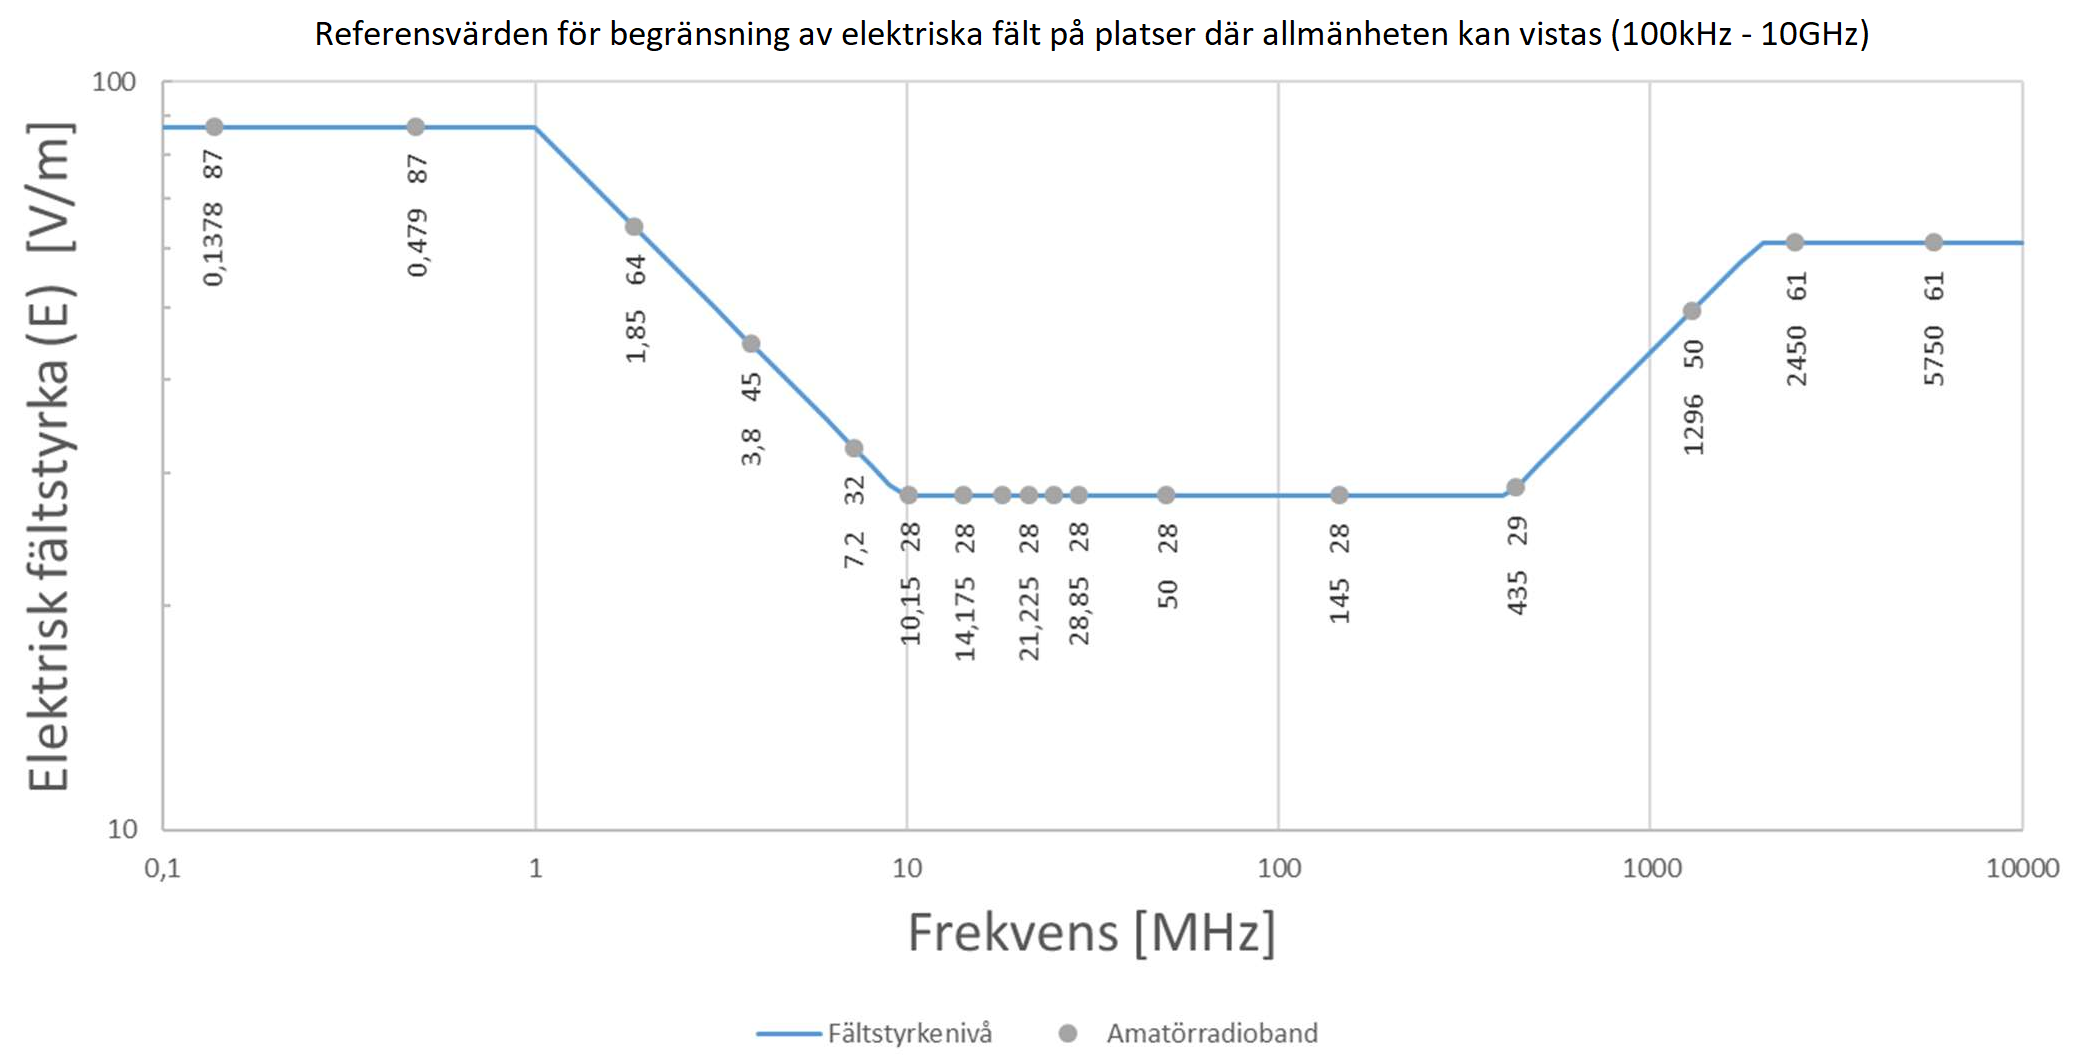
\includegraphics[width=\textwidth]{images/emfbild-000.png}
\end{figure}
\end{frame}

\section{Manuell beräkning av fältstyrka}

\begin{frame}{Faktorer för beräkning}
\begin{itemize}
	\item antennens förstärkning (G)
	\item sändningens medeleffekt (P)
	\item transmissionsledningens förluster (k)
	\item distansen (d)
\end{itemize}
\end{frame}

\begin{frame}{Antennens förstärkning (G)}
Antennens förstärkning ska anges i linjära termer i förhållande till en isotrop
antenn, dBi

\begin{tabular}{|l|ccccc|}
	\hline
	dB     &  0  & 2,15 &  3  &  6  &  9  \\ \hline
	G & 1,0 & 1,64 & 2,0 & 4,0 & 7,9 \\ \hline
	dB     &  10  &  12  &  15  &  18  &  20 \\ \hline
	G & 10,0 & 15,8 & 31,6 & 63,1 & 100 \\ \hline
\end{tabular}
\end{frame}

\begin{frame}{Sändningens medeleffekt (P)}

\(P_{medel} = P_{max} \cdot Modulationsfaktor \cdot Intermittensfaktor\)
\end{frame}

\begin{frame}{Modulationsfaktor}
\begin{tabular}{|l|c|}
	\hline
	Trafiksätt & Modulationsfaktor \\ \hline
	SSB & 0,2 \\ \hline
	CW & 0,4 \\ \hline
	SSB med processing & 0,5 \\ \hline
	FM & 1,0 \\ \hline
	MGM (t.ex. RTTY,PSK) & 1,0 \\ \hline
	Bärvåg & 1,0 \\ \hline
\end{tabular}
\end{frame}

\begin{frame}{Intermittensfaktor}
\begin{tabular}{|c|c|c|}
	\hline
	Sändning  & Mottagning & Intermittensfaktor \\
	(minuter) & (minuter)  & \\ \hline
	1 & 5 & 0,17 \\ \hline
	2 & 4 & 0,33 \\ \hline
	3 & 3 & 0,50 \\ \hline
	4 & 2 & 0,67 \\ \hline
	5 & 1 & 0,83 \\ \hline
	6 & 0 & 1,00 \\ \hline
\end{tabular}
\end{frame}

\begin{frame}{Kabeldämpning}
\begin{tabular}{|l|c|c|c|c|c|c|c|}
	\hline
	dB & 0,0  & 0,5  & 1,0  & 1,5  & 2,0  & 2,5  & 3,0 \\ \hline
	k  & 1,00 & 0,89 & 0,79 & 0,71 & 0,63 & 0,56 & 0,50 \\ \hline
\end{tabular}
\end{frame}

\begin{frame}{Förenklade formler}

\[ E=\dfrac{\sqrt{30 \cdot P \cdot G \cdot k}}{d}\qquad d=\dfrac{\sqrt{30 \cdot P \cdot G \cdot k}}{E}\]
\end{frame}

\section{Exempel}

\begin{frame}{Beräkning av säkerhetsavstånd}
En dipolantenn för \SI{3,75}{\mega\hertz} har jämfört med en isotrop antenn förstärkningen
\SI{2,15}{\decibel}i (cirka 1,6 gånger).
Max uteffekt är \SI{100}{\watt} och trafiksättet är SSB med normala TX/RX intervaller.
Den valda matarledningen har en dämpning på \SI{0,5}{\decibel} (0,89 gånger).
Referensvärdet för \SI{3,75}{\mega\hertz} är \SI{45}{\volt\per\meter}.
\end{frame}

\begin{frame}{Beräkning av säkerhetsavstånd}
\begin{itemize}
	\item \(P_{medel} = 100 \cdot 0,5 \cdot 0,5 = 25\, \mathrm{W}\) \vspace{4mm}
	\item \(G = 1,6 \quad k = 0,89 \quad E = 45\) \vspace{3mm}
	\item \(d = \dfrac{\sqrt{30 \cdot P \cdot G \cdot k}}{E} \Rightarrow \dfrac{\sqrt{30 \cdot 25 \cdot 1,6 \cdot 0,89}}{45} = 0,74\, \mathrm{m}\)
\end{itemize}
\end{frame}

\begin{frame}{Beräkning av säkerhetsavstånd}
\begin{itemize}
	\item För enkla antenner kan man ibland använda de förenklade formlerna för
	att uppskatta fältstyrka och säkerhetsavstånd även inom närfältet.
	\item För stora antenner med hög riktverkan eller små kompakta antenner går
	det inte enkelt att uppskatta fältstyrka. I dessa fall krävs mätningar eller
	beräkningar med antennanalysprogram
\end{itemize}
\end{frame}


\section{Beräkningsprogram}

\begin{frame}{Beräkningsprogram IcnirpCalc}

\begin{figure}[h]
	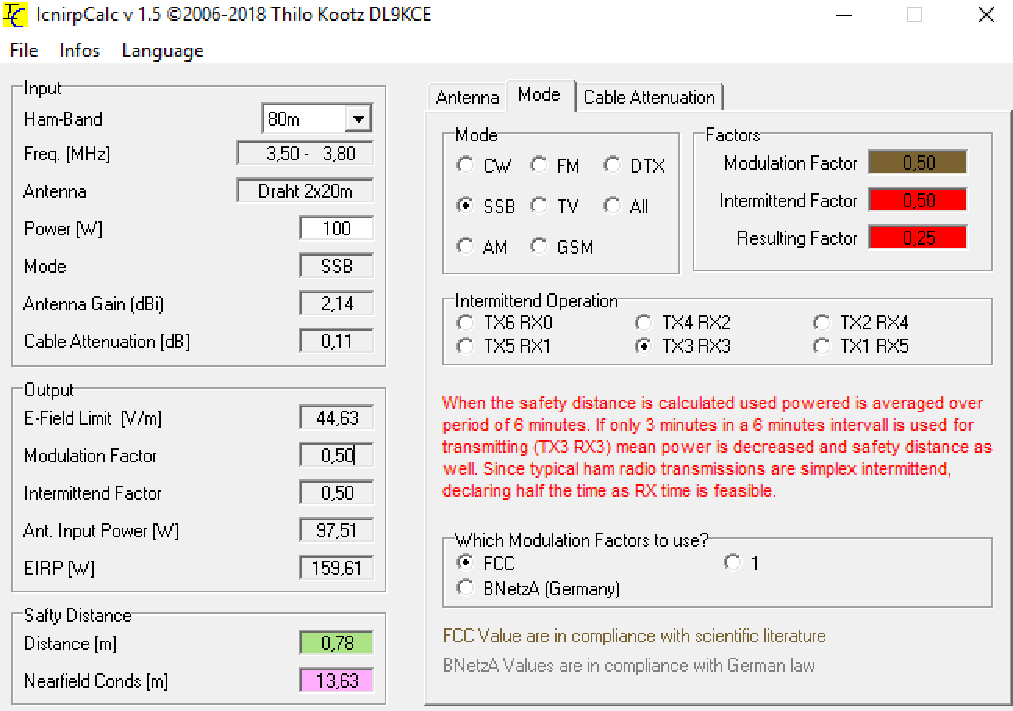
\includegraphics[width=0.8\textwidth]{images/IcnirpCalc.pdf}
\end{figure}

\end{frame}

\begin{frame}{Beräkningsprogram WattWächter}

\begin{figure}[h]
	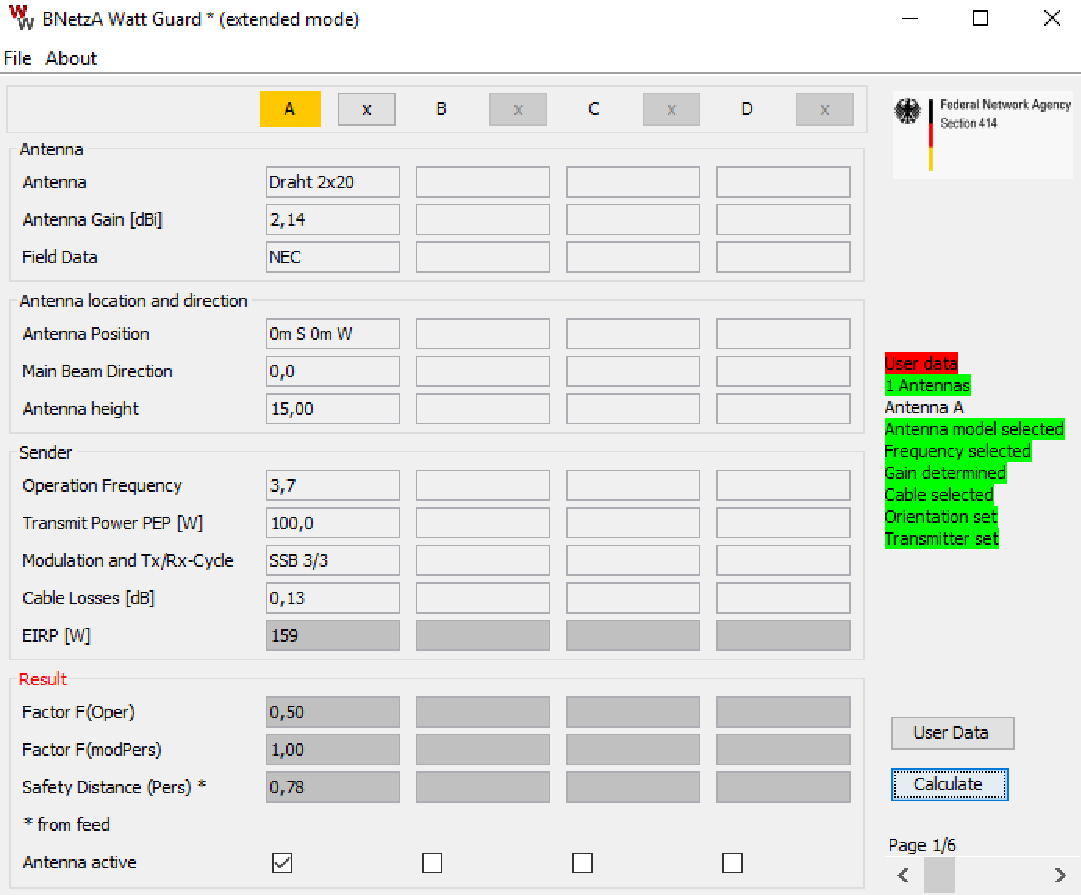
\includegraphics[width=0.8\textwidth]{images/Wattwaechter.pdf}
\end{figure}

\end{frame}

\section{Skyddsavstånd}

\begin{frame}{Skyddsavstånd dipol 80\,m 100\,W SSB}

\begin{figure}[h]

\includegraphics[width=\textwidth]{images/Dip_80m_100W_SSB_E_H_guard_area.pdf}
\end{figure}

\begin{itemize}
  \item skyddsavstånd i sidled \SI{0,78}{\meter}
  \item skyddsavstånd i längdled \SI{0,75}{\meter}
  \item i antennens mittre tredjedel dominerar det magnetiska fältet
  \item i antennens yttre tredjedelar dominerar det elektriska fältet
\end{itemize}
\end{frame}

\begin{frame}{Skyddsavstånd dipol 80\,m 1000\,W SSB}

\begin{figure}[h]
	
\includegraphics[width=\textwidth]{images/Dip_80m_1000W_SSB_E_H_guard_area.pdf}
\end{figure}

\begin{itemize}
	\item skyddsavstånd i sidled \SI{2,5}{\meter}
	\item skyddsavstånd i längdled \SI{2,2}{\meter}
	\item skyddsavstånd vid FM eller RTTY \SI{3,7}{\meter} respektive \SI{3,1}{\meter}
\end{itemize}
\end{frame}

\section{Andra begränsningar}

\begin{frame}{Krav på störtålighet EMC}

Utöver skyddskraven för människor så behöver vi även ta hänsyn till hur stor
fältstyrka en produkt tål.
\begin{itemize}
	\item generellt gäller \SI{3}{\volt\per\meter} för konsumentprodukter
\end{itemize}
Detta innebär att fältstyrkan vid sändning kan behöva minskas för att undvika
störningar på en konsumentprodukt som uppfyller kraven på störtålighet.
\end{frame}

\begin{frame}{Beräkning av separationsavstånd}

Om vi använder de tidigare exemplen och beräknar på vilket avstånd från antennen
(d) vi når den elektriska fältstyrkan \SI{3}{\volt\per\meter}
\begin{itemize}
	\item dipol \SI{80}{\meter} \SI{100}{\watt} SSB separationsavstånd \SI{11}{\meter}
	\item dipol \SI{80}{\meter} \SI{1000}{\watt} SSB separationsavstånd \SI{38}{\meter}
	\item dipol \SI{80}{\meter} \SI{1000}{\watt} FM eller RTTY separationsavstånd \SI{56}{\meter}
\end{itemize}
\end{frame}

\begin{frame}{Avslutningsvis}

\begin{itemize}
	\item det finns inget som säger att amatörer har rätt att använda fullt
	tillåten sändareffekt i alla lägen
	\item se inte stenhårt till principer
	\item undvik olämpliga antenner och antennplaceringar
\end{itemize}
\end{frame}

\section{Frågor}

\begin{frame}{Frågor}

\begin{itemize}
	\item ?
	\item ?
	\item ?
\end{itemize}
\end{frame}

\end{document}
